\chapter[SCP-139 疑似白魔的头骨]{
    SCP-139 Possible Skull of the White Div\\
    SCP-139 疑似白魔的头骨
}

\label{chap:SCP-139}

\begin{figure}[H]
    \centering
    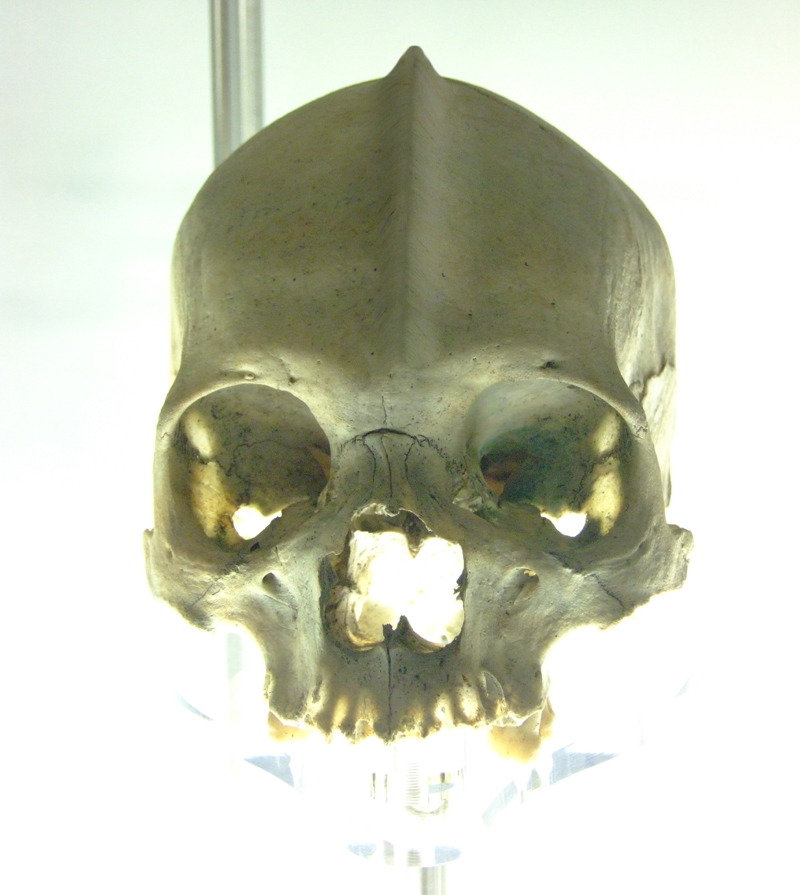
\includegraphics[width=0.5\linewidth]{images/SCP.139.jpg}
    \caption*{SCP-139}
\end{figure}

\bb{项目编号:}SCP-139

\bb{项目等级:}Keter

\bb{特殊收容措施:}SCP-139被悬挂在一个最小至少为六米的房间内,距房间内表面至少两米。在任何情况下所有人员都不得进入房间。房间随时要留有至少两名武装警卫进行看守。

\bb{描述:}对象在表面上至少是一枚保存不当的人类头骨。它缺少下颚骨。同样要注意到的是极度的磨损,特别是眼窝部分。

头骨的照片由领先的人类学家们进行了分析。所有人都认为该标本的损坏过于严重而不能完全确定,而极有可能是人类。然而有些人认为它是一颗标准的尼安德特人头骨,而其他人认为腔窝的宽度是受到磨损的结果,而原始尺寸要小得多,所以更可能是一名现代人类。这是由于根据鼻腔于眼窝的大小为主要特征进行判断,导致一些人认为这是一枚尼安德特人头骨。然而,所有人都为颅骨顶部凸起的脊所迷惑。此特征最常见于史前的草食性人类。

我们的一名人类学家提出的理论是,脊是具有强有力下颚的动物的特征。这类脊通常是作为颌骨肌肉的固定点,例如鲍氏傍人(\ii{Paranthropus boisei})。这些动物用它们那沉重的颌骨肌肉来咀嚼植物,但这同样可以在具有锋利的牙齿的情况下轻易地用于杀戮。

以下部分由████ █ █████博士根据ORIA文件D.TDL67翻译。

\begin{scpbox}

\ii{头骨在位于贾姆希德王权(Throne of Jamshid)南面的一个小镇上被发现。}{[}Takht-e Jamshid,或“Throne of Jamshid”被确定为波塞波利斯的现代波斯语名称。]

\ii{头骨首次被记载是由Douglas Winthrop,一名英国人,盎格鲁-伊朗石油公司(Anglo-Iranian Oil)雇员,在1370s。}{[}大约是公历20世纪50年代]\ii{Winthrop是一名追求名利与荣誉的业余人类学家,在到达小镇后他希望找到一个生活中缺失的环节。他认为小镇的居民中可能存在尼安德特人。不过在对镇上居民进行检查后这个假设很快就被放弃,他没有发现头骨。}

\ii{在发现时,头骨被放在一个有铁和铜制成的笼子里,用麻绳吊在距悬崖五十英尺}{[}15.24米]\ii{的空中。绳子被绑在钻在悬崖边的一个钩子上,这意味着并不打算把它收回来。然而,那里有一个滑轮。它被挂在一堵竖立在悬崖边的墙上。滑轮是用来向头骨处放下食物和水的。}

\ii{人们将头骨称作白魔的头骨(the skull of the White Div)。在古老的传说中,白魔是一个恶魔,并且是所有罪恶的集合,Ahriman的产物。传说中具有庞大而神秘的力量的白魔被Rostam击败。}{[}Rostam是波斯的传奇英雄]\ii{据称魔鬼在现在阿塞拜疆的北部山区中被杀死。}

\ii{按照镇上居民的说法,头骨是被一个杀害了许多人的疯子带到镇上的,随后他们发现了头骨所承载的力量并把它放到了现在地方。}

\end{scpbox}

Winthrop很快被自己的疯狂所占据,他在回到英格兰后杀害了自己的七个朋友。他还受到鸡奸若干雄性和雌性动物(其中包括若干只鸡,雄性和雌性的狗各一,以及三头公牛)的指控并定罪。

然而,由于头骨被沙哈政权下的设立子大学(University of Shiraz)没收,他没能将头骨带回来。

然而在被没收后,没有再对它进行新的研究。

物品在距阿拉斯加九十公里的育空地区边缘浮出水面。加拿大驯鹿十字(即当今的育空地区的卡克罗斯)的整个社区被发现遭到了残忍的杀害,尸体上有多处刀伤。在伤口中发现了精液,并推测是行凶者向伤口中射精。尸体被发现堆放在教堂的中心。而置于尸堆顶端的则是这枚头骨。

从那以后该物品一直处于我们的监管下。

其属性是未知的。不知道是什么在它影响下驱使了这类迷信活动。不知道是什么把它带到了剧烈的大屠杀现场。目前所采取的安全预防措施只是因为迄今为止这被证明是有效的。不知道是为什么。

没有研究计划。

\bb{另见:}\\
\hyperref[sec:DOC-personal-journal-of-douglas-winthrop]{Douglas Winthrop的个人日记}

\newpage
\section{Douglas Winthrop的个人日记}

\label{sec:DOC-personal-journal-of-douglas-winthrop}

\bb{个人日志:}Douglas Winthrop, b. 1918

\bb{日期:06-15-1950}

我们几乎已经到了法尔斯地区的扎尔甘(Zargan, Fars Province)。从波斯湾出发开始就一直受到东方共产主义者(或者他们更愿意被称为“民族主义者”)的困扰,他们声称这片土地上的家庭和不发达国家的经济纷争拒绝一个更发达的国家的人的指导。

作为一个在这片蛮荒土地上的英国人,收集在法国发现的现代人与古代类人猿的化石证据之间可能缺失的考古证据是我的责任。我最大的希望是在扎尔甘找到一个存在缺失的环节。

最古怪的事情发生在从设拉子出发的路上。我们的汽车受到一名皮肤异常苍白的男子的猛烈袭击。我可能说过我从他那充满血丝的眼睛中看出他吸食了当地的大麻或鸦片,然而他提出了抢占能源这一概念。当这名男子从灌木丛后面冲出来并追赶我们时,我们正以超过每小时五十公里的速度行驶着。他几乎追上了汽车,并朝我们投掷石块。不过我们仅仅受了点皮外伤,事故真是多发。

也许这是来自我们未来的恶魔。当我们接近目的地时我发现肚子上有一个病态的肿块,我感到一股恶寒爬上了脊柱。这有什么可害怕的呢?我已经在伊朗生活了两年,和这些东方人相处了近十年。

我们在一天内到达。

\bb{注:}见:\hyperref[chap:SCP-139]{SCP-139}

